%%%%%%%%%%%%%%%%%%%%%%%%%%%%%%%%%%%%%%%%%
% Lachaise Assignment
% LaTeX Template
% Version 1.0 (26/6/2018)
%
% This template originates from:
% http://www.LaTeXTemplates.com
%
% Authors:
% Marion Lachaise & François Févotte
% Vel (vel@LaTeXTemplates.com)
%
% License:
% CC BY-NC-SA 3.0 (http://creativecommons.org/licenses/by-nc-sa/3.0/)
% 
%%%%%%%%%%%%%%%%%%%%%%%%%%%%%%%%%%%%%%%%%

%----------------------------------------------------------------------------------------
%	PACKAGES AND OTHER DOCUMENT CONFIGURATIONS
%----------------------------------------------------------------------------------------

\documentclass{article}

%%%%%%%%%%%%%%%%%%%%%%%%%%%%%%%%%%%%%%%%%
% Lachaise Assignment
% Structure Specification File
% Version 1.0 (26/6/2018)
%
% This template originates from:
% http://www.LaTeXTemplates.com
%
% Authors:
% Marion Lachaise & François Févotte
% Vel (vel@LaTeXTemplates.com)
%
% License:
% CC BY-NC-SA 3.0 (http://creativecommons.org/licenses/by-nc-sa/3.0/)
% 
%%%%%%%%%%%%%%%%%%%%%%%%%%%%%%%%%%%%%%%%%

%----------------------------------------------------------------------------------------
%	PACKAGES AND OTHER DOCUMENT CONFIGURATIONS
%----------------------------------------------------------------------------------------

\usepackage{amsmath,amsfonts,stmaryrd,amssymb} % Math packages

\usepackage{enumerate} % Custom item numbers for enumerations

\usepackage[ruled]{algorithm2e} % Algorithms

\usepackage[framemethod=tikz]{mdframed} % Allows defining custom boxed/framed environments

\usepackage{listings} % File listings, with syntax highlighting
\lstset{
	basicstyle=\ttfamily, % Typeset listings in monospace font
}

%----------------------------------------------------------------------------------------
%	DOCUMENT MARGINS
%----------------------------------------------------------------------------------------

\usepackage{geometry} % Required for adjusting page dimensions and margins

\geometry{
	paper=a4paper, % Paper size, change to letterpaper for US letter size
	top=2.5cm, % Top margin
	bottom=3cm, % Bottom margin
	left=2.5cm, % Left margin
	right=2.5cm, % Right margin
	headheight=14pt, % Header height
	footskip=1.5cm, % Space from the bottom margin to the baseline of the footer
	headsep=1.2cm, % Space from the top margin to the baseline of the header
	%showframe, % Uncomment to show how the type block is set on the page
}

%----------------------------------------------------------------------------------------
%	FONTS
%----------------------------------------------------------------------------------------

\usepackage[utf8]{inputenc} % Required for inputting international characters
\usepackage[T1]{fontenc} % Output font encoding for international characters

\usepackage{XCharter} % Use the XCharter fonts

%----------------------------------------------------------------------------------------
%	COMMAND LINE ENVIRONMENT
%----------------------------------------------------------------------------------------

% Usage:
% \begin{commandline}
%	\begin{verbatim}
%		$ ls
%		
%		Applications	Desktop	...
%	\end{verbatim}
% \end{commandline}

\mdfdefinestyle{commandline}{
	leftmargin=10pt,
	rightmargin=10pt,
	innerleftmargin=15pt,
	middlelinecolor=black!50!white,
	middlelinewidth=2pt,
	frametitlerule=false,
	backgroundcolor=black!5!white,
	frametitle={Command Line},
	frametitlefont={\normalfont\sffamily\color{white}\hspace{-1em}},
	frametitlebackgroundcolor=black!50!white,
	nobreak,
}

% Define a custom environment for command-line snapshots
\newenvironment{commandline}{
	\medskip
	\begin{mdframed}[style=commandline]
}{
	\end{mdframed}
	\medskip
}

%----------------------------------------------------------------------------------------
%	FILE CONTENTS ENVIRONMENT
%----------------------------------------------------------------------------------------

% Usage:
% \begin{file}[optional filename, defaults to "File"]
%	File contents, for example, with a listings environment
% \end{file}

\mdfdefinestyle{file}{
	innertopmargin=1.6\baselineskip,
	innerbottommargin=0.8\baselineskip,
	topline=false, bottomline=false,
	leftline=false, rightline=false,
	leftmargin=2cm,
	rightmargin=2cm,
	singleextra={%
		\draw[fill=black!10!white](P)++(0,-1.2em)rectangle(P-|O);
		\node[anchor=north west]
		at(P-|O){\ttfamily\mdfilename};
		%
		\def\l{3em}
		\draw(O-|P)++(-\l,0)--++(\l,\l)--(P)--(P-|O)--(O)--cycle;
		\draw(O-|P)++(-\l,0)--++(0,\l)--++(\l,0);
	},
	nobreak,
}

% Define a custom environment for file contents
\newenvironment{file}[1][File]{ % Set the default filename to "File"
	\medskip
	\newcommand{\mdfilename}{#1}
	\begin{mdframed}[style=file]
}{
	\end{mdframed}
	\medskip
}

%----------------------------------------------------------------------------------------
%	NUMBERED QUESTIONS ENVIRONMENT
%----------------------------------------------------------------------------------------

% Usage:
% \begin{question}[optional title]
%	Question contents
% \end{question}

\mdfdefinestyle{question}{
	innertopmargin=1.2\baselineskip,
	innerbottommargin=0.8\baselineskip,
	roundcorner=5pt,
	nobreak,
	singleextra={%
		\draw(P-|O)node[xshift=1em,anchor=west,fill=white,draw,rounded corners=5pt]{%
		Question \theQuestion\questionTitle};
	},
}

\newcounter{Question} % Stores the current question number that gets iterated with each new question

% Define a custom environment for numbered questions
\newenvironment{question}[1][\unskip]{
	\bigskip
	\stepcounter{Question}
	\newcommand{\questionTitle}{~#1}
	\begin{mdframed}[style=question]
}{
	\end{mdframed}
	\medskip
}

%----------------------------------------------------------------------------------------
%	WARNING TEXT ENVIRONMENT
%----------------------------------------------------------------------------------------

% Usage:
% \begin{warn}[optional title, defaults to "Warning:"]
%	Contents
% \end{warn}

\mdfdefinestyle{warning}{
	topline=false, bottomline=false,
	leftline=false, rightline=false,
	nobreak,
	singleextra={%
		\draw(P-|O)++(-0.5em,0)node(tmp1){};
		\draw(P-|O)++(0.5em,0)node(tmp2){};
		\fill[black,rotate around={45:(P-|O)}](tmp1)rectangle(tmp2);
		\node at(P-|O){\color{white}\scriptsize\bf !};
		\draw[very thick](P-|O)++(0,-1em)--(O);%--(O-|P);
	}
}

% Define a custom environment for warning text
\newenvironment{warn}[1][Warning:]{ % Set the default warning to "Warning:"
	\medskip
	\begin{mdframed}[style=warning]
		\noindent{\textbf{#1}}
}{
	\end{mdframed}
}

%----------------------------------------------------------------------------------------
%	INFORMATION ENVIRONMENT
%----------------------------------------------------------------------------------------

% Usage:
% \begin{info}[optional title, defaults to "Info:"]
% 	contents
% 	\end{info}

\mdfdefinestyle{info}{%
	topline=false, bottomline=false,
	leftline=false, rightline=false,
	nobreak,
	singleextra={%
		\fill[black](P-|O)circle[radius=0.4em];
		\node at(P-|O){\color{white}\scriptsize\bf i};
		\draw[very thick](P-|O)++(0,-0.8em)--(O);%--(O-|P);
	}
}

% Define a custom environment for information
\newenvironment{info}[1][Info:]{ % Set the default title to "Info:"
	\medskip
	\begin{mdframed}[style=info]
		\noindent{\textbf{#1}}
}{
	\end{mdframed}
}
 % Include the file specifying the document structure and custom commands

%----------------------------------------------------------------------------------------
%	ASSIGNMENT INFORMATION
%----------------------------------------------------------------------------------------

\title{Examen de Computación II} % Title of the assignment

\author{Abel Rosado Peinado - 5265\\ \texttt{abel.rosado@estudiante.uam.es}} % Author name and email address

\date{UAM --- \today} % University, school and/or department name(s) and a date

%----------------------------------------------------------------------------------------

\begin{document}

\maketitle % Print the title

\section*{Ejercicio 1}
\subsection*{a. Introducción al problema}
El problema consiste en hallar los ceros de la siguiente función, 
\[f(\lambda) = \lambda^{-1/2}+2 \log_{10}{\left(\frac{2.51}{\lambda^{1/2} R_e}+ \frac{K}{3.71D}\right)},\]
para $K=0.25\cdot10^{-3}$ m, $D = 0.3$ m y $R_e = 200000$.

Si representamos la función, como se observa en la siguiente figura, podemos apreciar visualmente que esta corta el 0 aproximadamente en $\lambda \approx 0.02$.

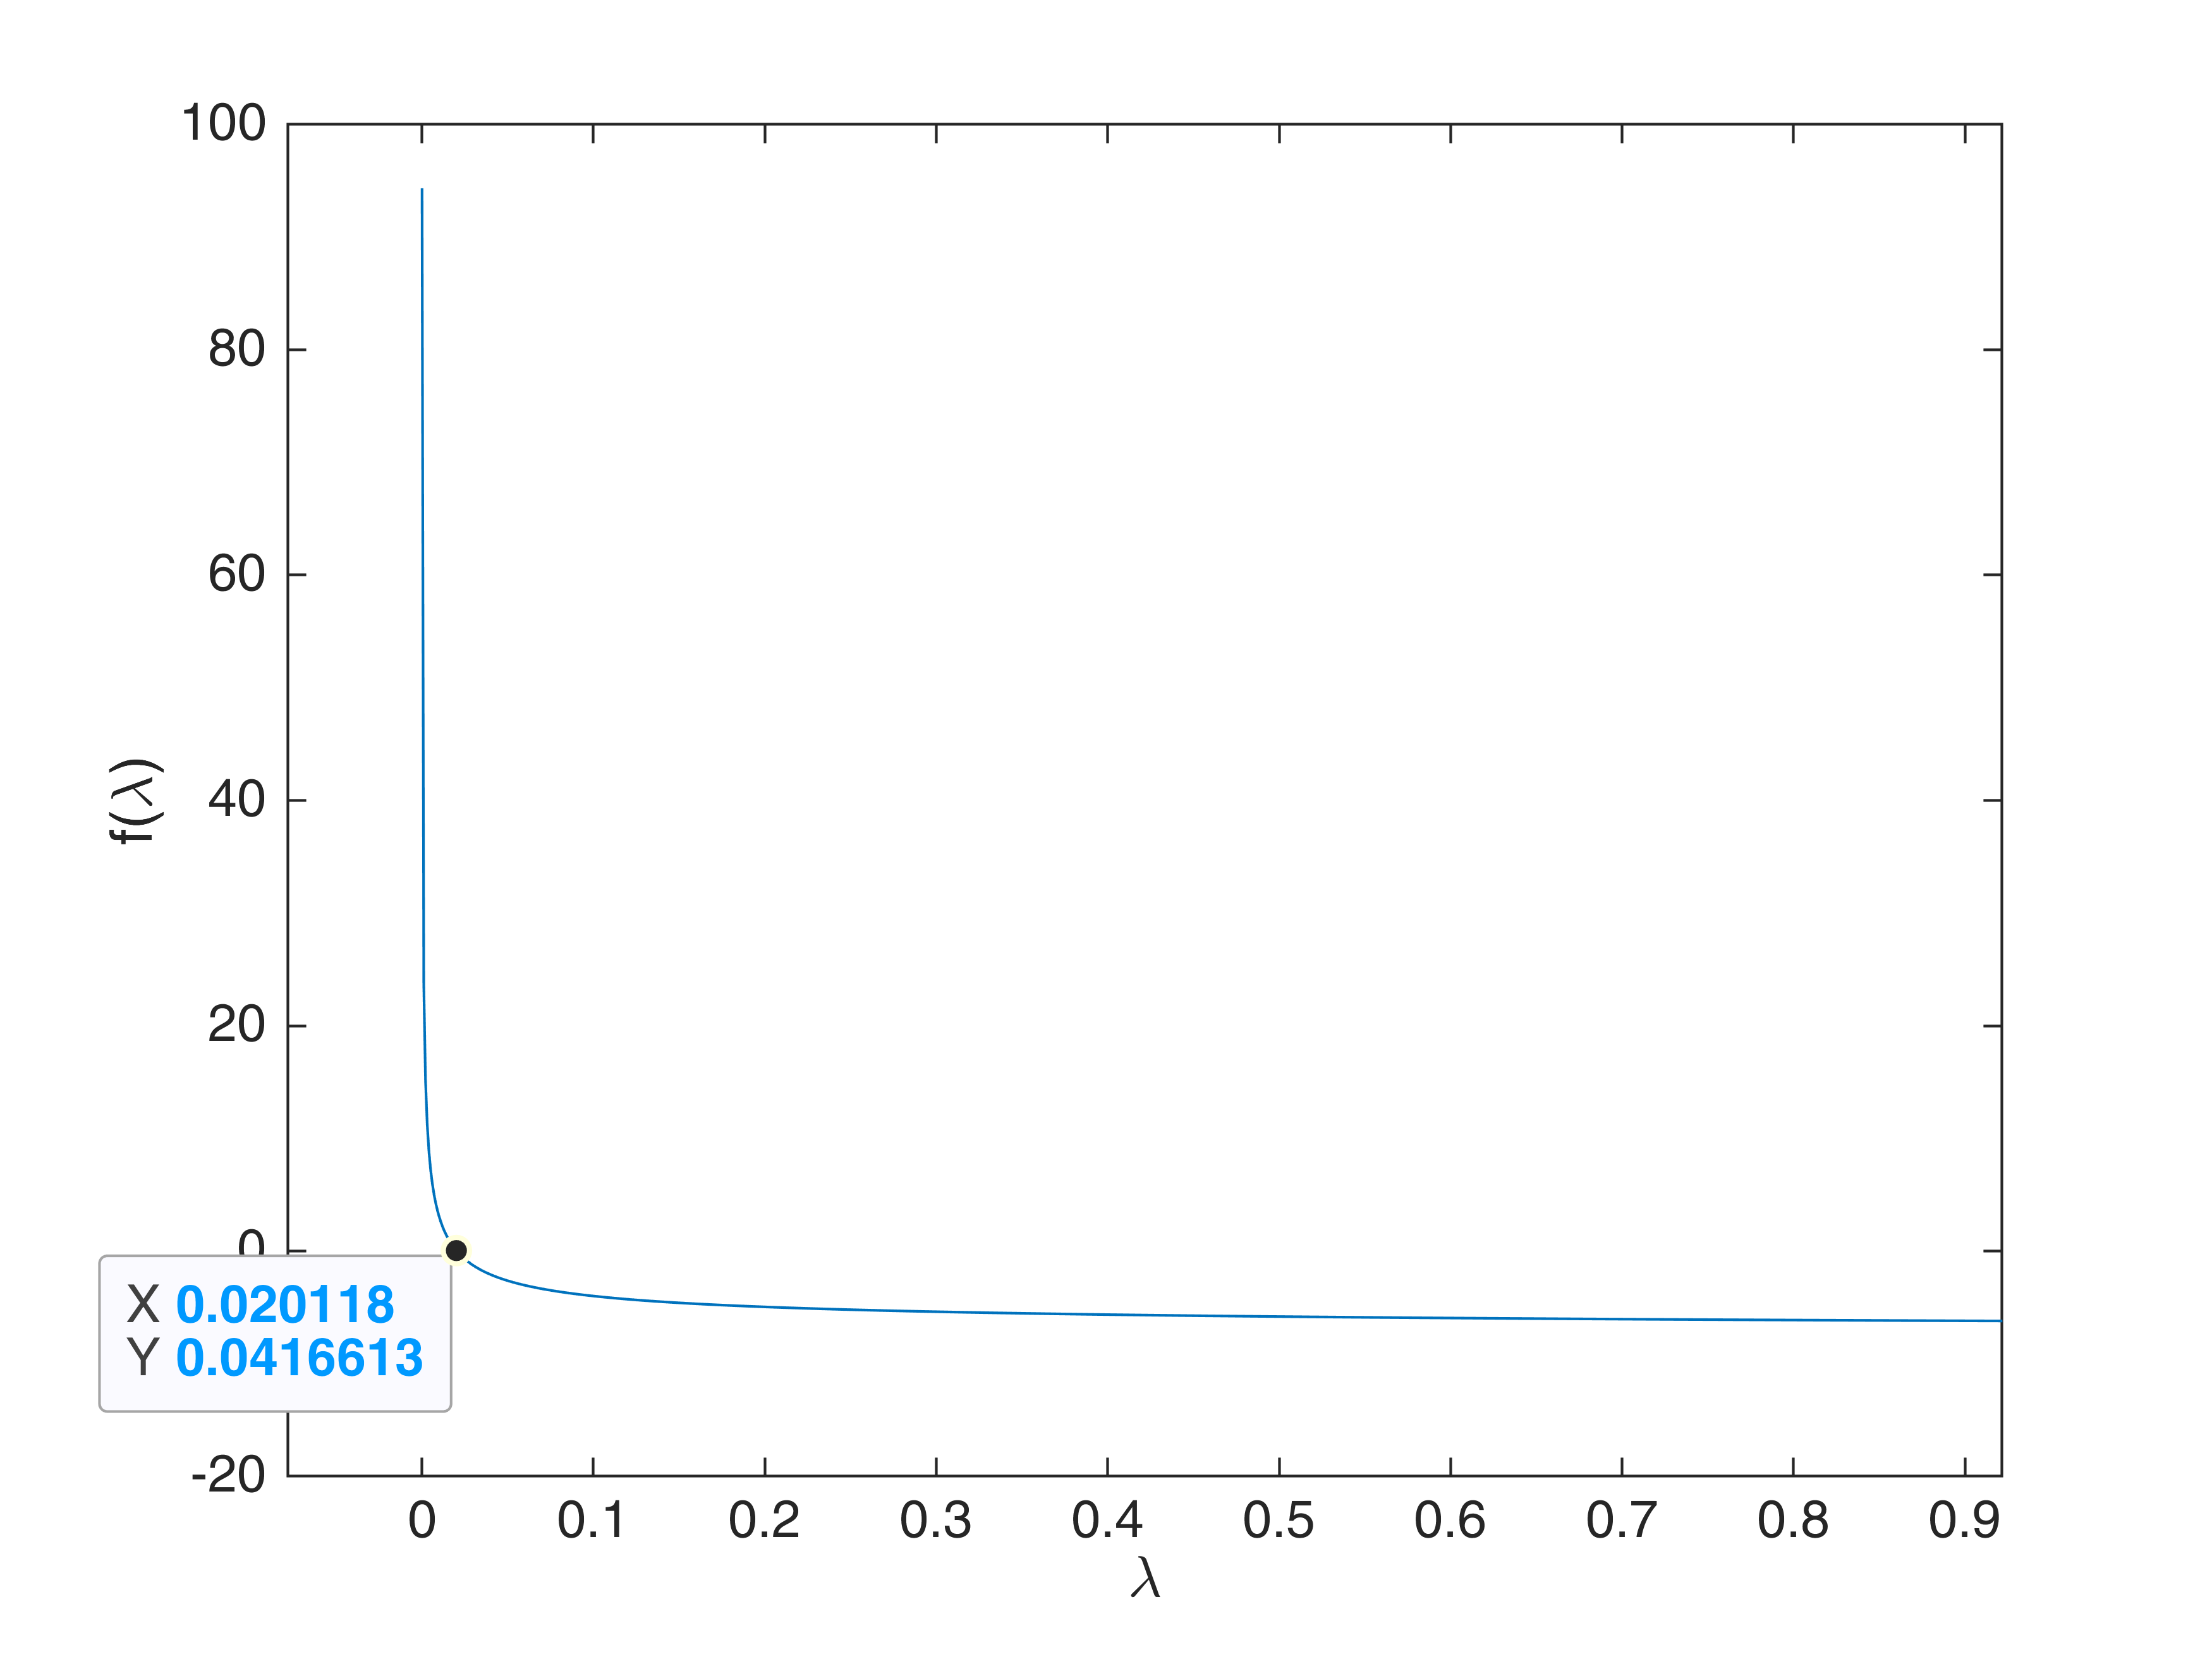
\includegraphics{untitled1.png}

\subsection*{b. Bisección y Newton-Rhapson}
Para determinar más concretamente cual es esa raiz, usaremos el método de la bisección en el intervalo $\lambda \in [0.0001,1]$ y el método de Newton-Rhapson con punto inicial $\lambda = 0.0001$, calculando la derivada de forma numérica con $h$ igual a la tolerancia, como estamos utilizando las diferencias centradas, sabemos que el error de ese método es de orden $h^2$, por lo que el error cometido al hacer la derivada numérica será muchísimo menor a la tolerancia.

Hemos establecido una tolerancia de $10^{-9}$ para obtener en ambos métodos unas soluciones con una precisión de 8 cifras significativas.
\[\lambda_{\mbox{\small bisección}} = 0.020349756 \ \ \ \ \ \ \lambda_{\mbox{\small Newton}} = 0.020349756\]
Observamos que obtenemos el mismo resultado en ambos métodos, y que concuerdan con el resultado que cabría esperar tras la inspección visual, por lo que podemos estar bastante seguros que no nos hemos equivocado.

Los dos métodos se diferencian en el número de iteraciones que tardan en completarse, mientras que el método de la bisección tarda 30 iteraciones en alcanzar la precisión establecida, el método de Newton-Rhapson lo logra en tan solo 11 iteraciones.

Tenemos una expresión que nos estima el número iteraciones necesario para alcanzar la raiz utilizando el método de la bisección con una precisión dada en un intervalo inicial dado, tal que 
\[n \geq \left\lceil \log_2{\frac{b-a}{\epsilon}}\right\rceil = \left\lceil \log_2{\frac{1-0.0001}{10^{-9}}}\right\rceil =\left\lceil 29.8972\right\rceil =  30\]
Mientras que el método de la bisección es de orden lineal, el método de Newton-Rhapson es cuadrático, por lo que es esperable que requiera muchas menos iteraciones que el de la bisección.

\subsection*{c. Secante}
Por otro lado, podríamos intentar usar el método de la secante en el mismo intervalo que el método de la bisección, pero este va a fallar por lo que se observa en la siguiente figura

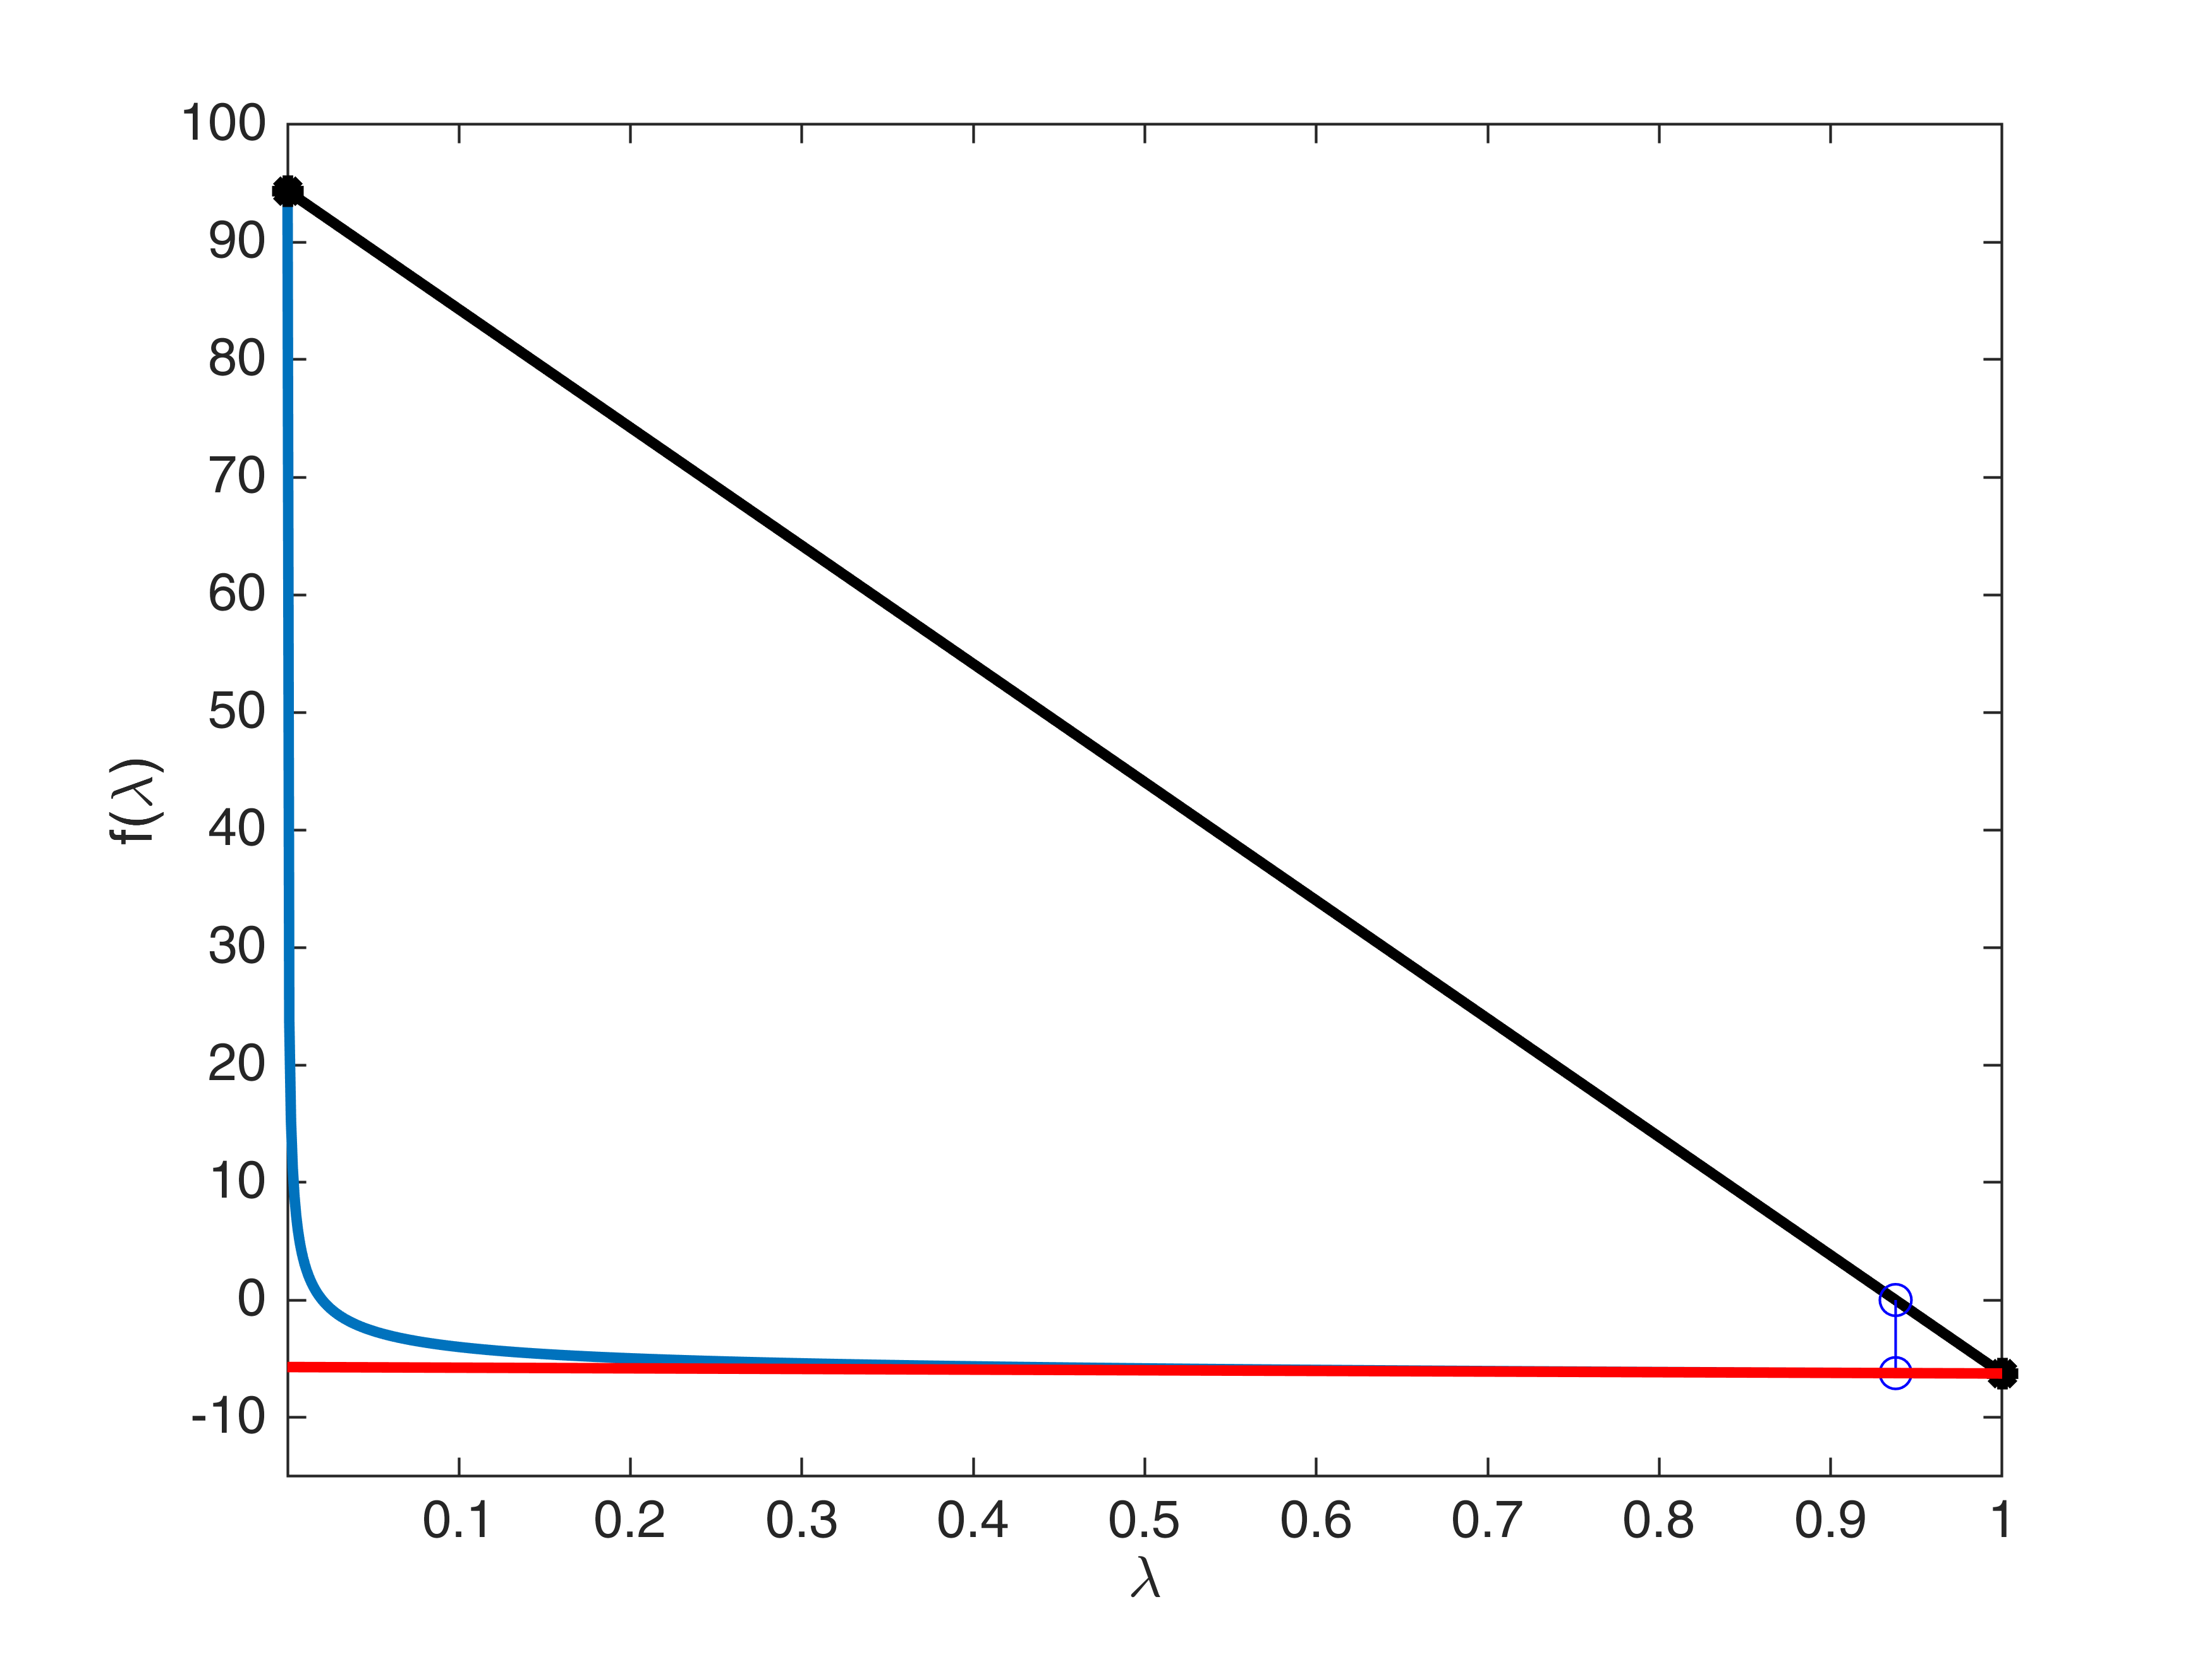
\includegraphics{untitled.png}

En la primera iteración, la recta corta el eje x en $\lambda \approx 0.94$, tal que $f(0.94) \approx -6.216$, y en la segunda iteración, la recta resultante corta el eje x en $\lambda \approx -10.39$, donde la función no esta definida, por lo que el método falla.
\newpage
\section*{Ejercicio 2}
\subsection*{a. Construir matriz}
Podemos escoger cualquier matriz invertible, pero nos conviene elegir una matriz que no tenga 0s en la diagonal para poder pivotar en el método LU y no tener que cambiar las filas, y además que sea diagonalmente dominante, para asegurarnos la convergencia con los métodos de Jacobi y Gauss-Seidel.
\[\mathbf{A} = \left[\begin{matrix}
10 & 1 & 1 & 1 & 1 & 1 & 1 & 1 & 1 & 0 \\
1 & 10 & 1 & 1 & 1 & 1 & 1 & 1 & 0 & 1 \\
1 & 1 & 10 & 1 & 1 & 1 & 1 & 0 & 1 & 1 \\
1 & 1 & 1 & 10 & 1 & 1 & 0 & 1 & 1 & 1 \\
1 & 1 & 1 & 1 & 10 & 0 & 1 & 1 & 1 & 1 \\
1 & 1 & 1 & 1 & 0 & 10 & 1 & 1 & 1 & 1 \\
1 & 1 & 1 & 0 & 1 & 1 & 10 & 1 & 1 & 1 \\
1 & 1 & 0 & 1 & 1 & 1 & 1 & 10 & 1 & 1 \\
1 & 0 & 1 & 1 & 1 & 1 & 1 & 1 & 10 & 1 \\
0 & 1 & 1 & 1 & 1 & 1 & 1 & 1 & 1 & 10 
\end{matrix}\right]\ \ \ \ \ \ \mathbf{b} = \left[\begin{matrix}
	0 \\
	1 \\
	2 \\
	3 \\
	4 \\
	5 \\
	6 \\
	7 \\
	8 \\
	9 
	\end{matrix}\right]\ \ \ \ \ \ \mathbf{A} \mathbf{x} = \mathbf{b}\]
Como $\mathbf{A}$ es simétrica, podemos diagonalizarla utilizando el método de jacobi, y podemos comprobar que su determinante es no nulo, concretamente $\det(\mathbf{A}) = 10^{10} \pm 10^{-8}$, y por lo tanto es invertible y el sistema propuesto tiene solución.
\subsection*{b. LU}
Utilizando entonces el método LU para obtener la solución al sistema tenemos la siguiente solución, que podemos verificar haciendo el producto matricial que es correcta.
\[\mathbf{x}_{\mbox{\small LU}}^T = \left[\begin{matrix}
	-0.2 & -0.1 & 0 & 0.1 & 0.2 & 0.3 & 0.4 & 0.5 & 0.6 & 0.7
\end{matrix}\right]\]

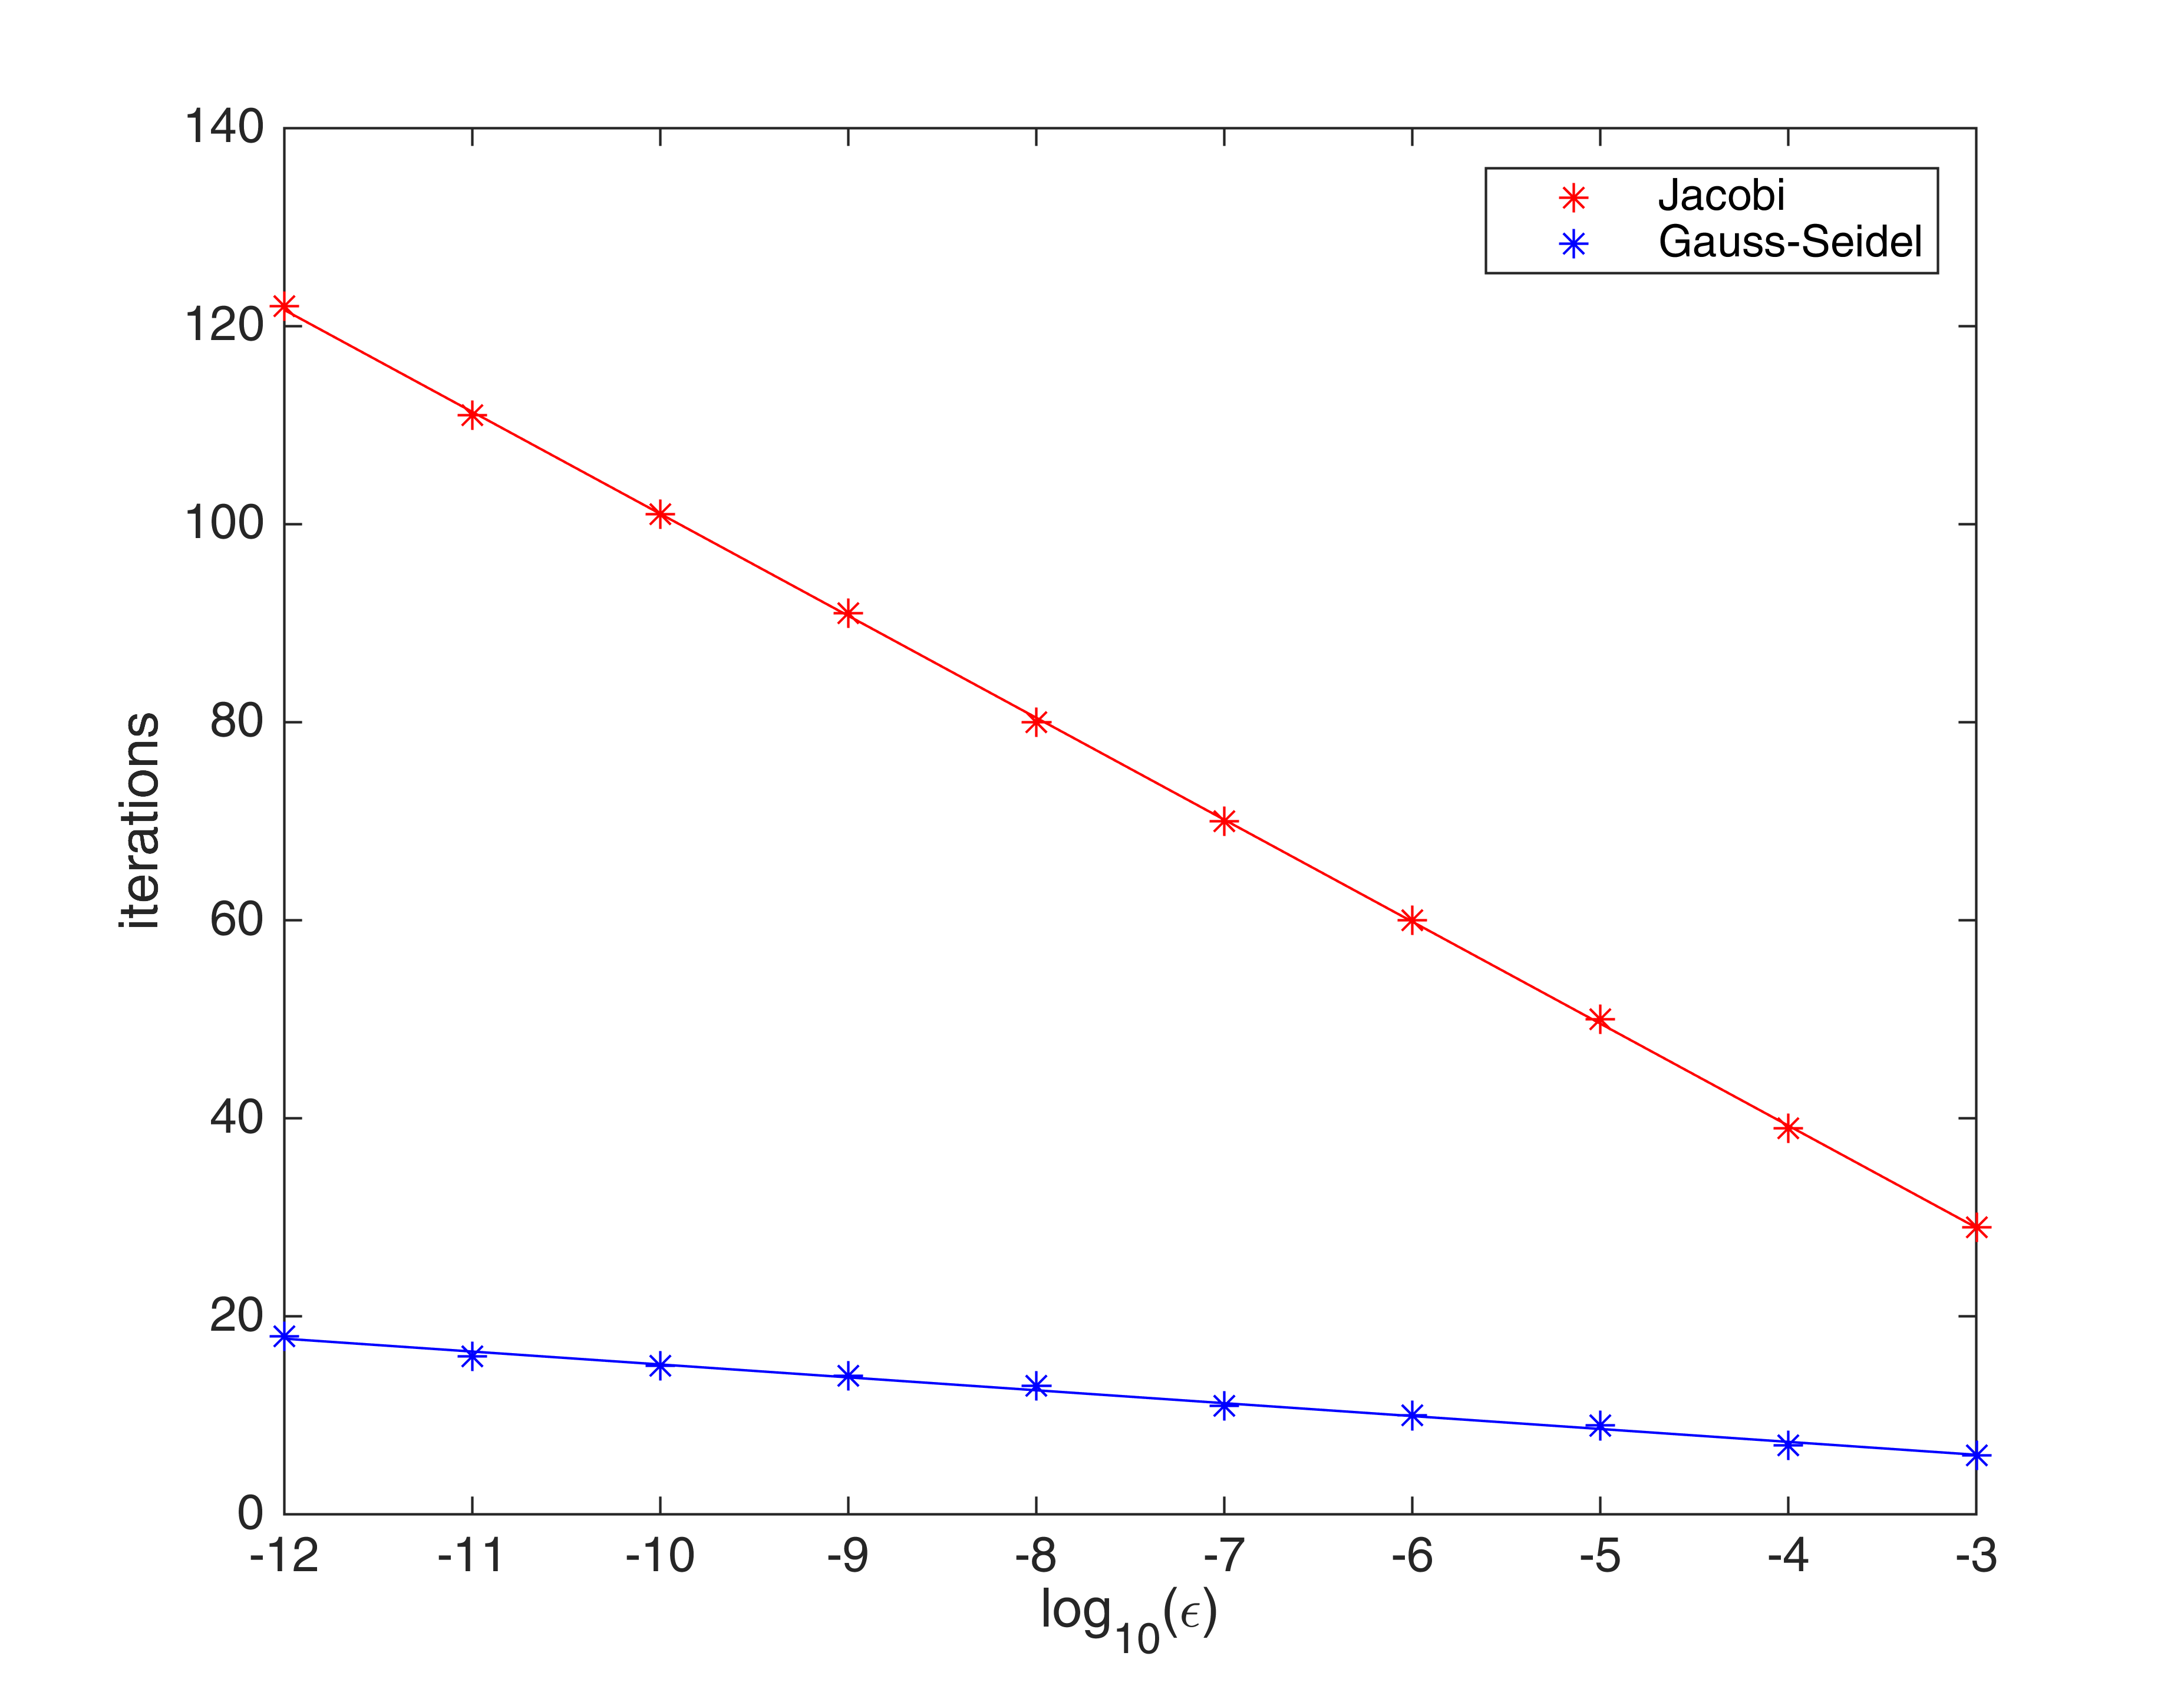
\includegraphics{untitled2.png}

\subsection*{c. Métodos iterativos}
Ahora entonces resolvemos el sistema anterior utilizando los métodos de Jacobi y Gauss-Seidel para precisiones que varían por múltiplos de $10^{-1}$ desde $10^{-3}$ hasta $10^{-12}$, para determinar el error en cada iteración he utilizado la norma suprema, comprobando si $||\mathbf{x}^i-\mathbf{x}^{i-1}||_\infty = \max\left(|x_j^i-x_j^{i-1}|\right) < \epsilon$.

No creo que sea informativo poner el resultado de cada precisión para cada método, así que daré los resultados para la precisión final de $10^{-12}$, que nos salen idénticas al resultado anterior, salvo por un error de orden $10^{-12}$.
\[\mathbf{x}_{\mbox{\small Jacobi}}^T = \left[\begin{matrix}
	-0.2 & -0.1 & 0 & 0.1 & 0.2 & 0.3 & 0.4 & 0.5 & 0.6 & 0.7
\end{matrix}\right]\]
\[\mathbf{x}_{\mbox{\small Gauss-Seidel}}^T = \left[\begin{matrix}
	-0.2 & -0.1 & 0 & 0.1 & 0.2 & 0.3 & 0.4 & 0.5 & 0.6 & 0.7
\end{matrix}\right]\]
Entonces ahora representamos el número de iteraciones que toma cada método para hallar la solución a una precisión determinada en función de esa precisión, que se observa en la figura de la página anterior.

Se observa entonces que el método de Gauss-Seidel es mucho más rápido que el de Jacobi, necesitando entre 5 y 7 veces menos iteraciones, al menos para esta matriz en concreto.


Se observa además que hay una relación lineal en ambos casos entre el número de iteraciones y $log_{10}(\epsilon)$. Podemos hacer un ajuste por mínimos cuadrados como se observa en la figura y obtenemos unas pendientes
\[m_{\mbox{\small Gauss-Seidel}} \approx -1.3 \mbox{ iteraciones} \ \ \ \ \ \ m_{\mbox{\small Jacobi}} \approx -10.3 \mbox{ iteraciones}\]
\end{document}
